\section{Methods} \label{sec:methods}

This section will introduce the strategy of our hereditary stratigraph approach to decentralized phylogenetic tracking, define the vocabulary we developed to describe aspects of this approach, overview configuration options of the approach, perform mathematical exposition of the properties of the approach under particular configurations, and then recap digital experiments that demonstrate this approach in an applied setting.

\subsection{Hereditary Strata and the Hereditary Stratigraphic Column}

\begin{figure}
    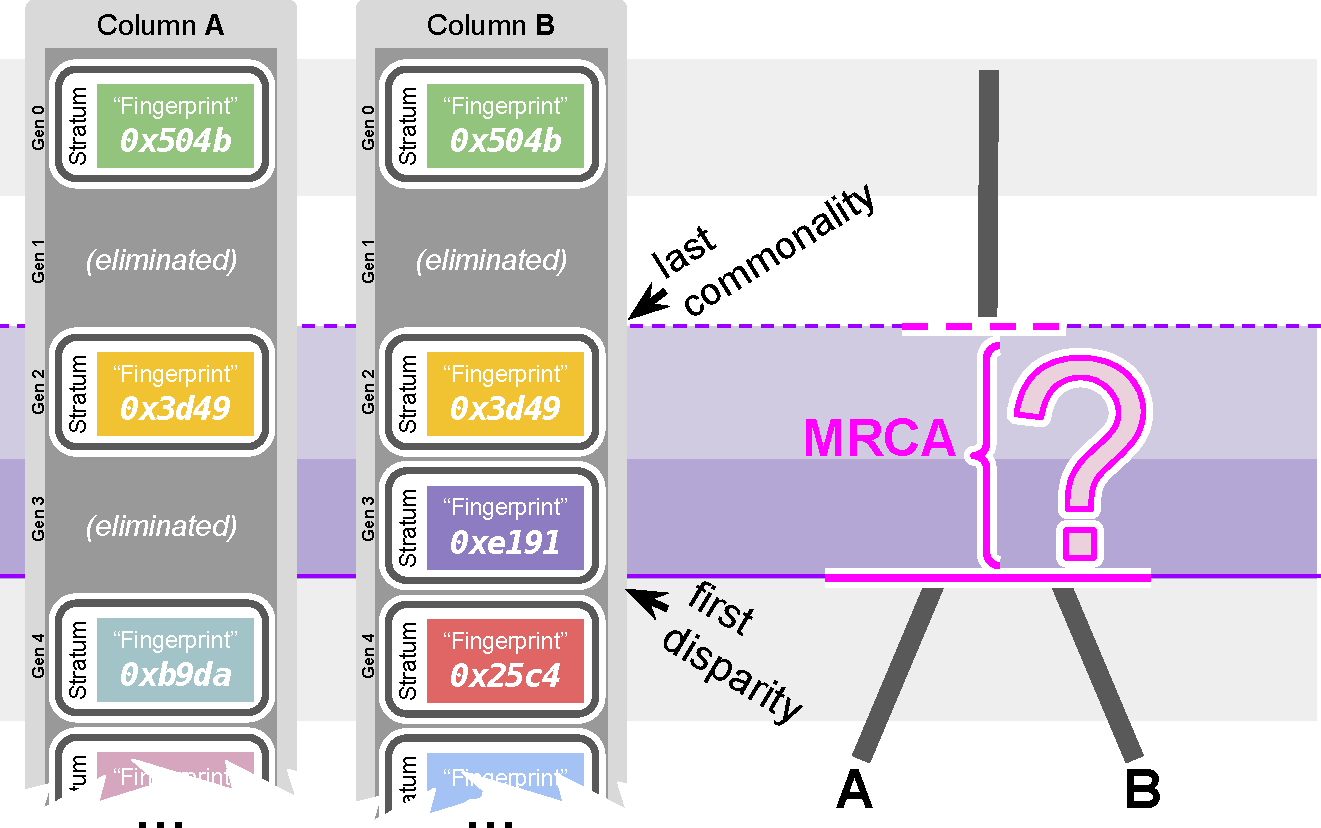
\includegraphics[width=\columnwidth]{img/column-comparison}
    \caption{
    Inferring the generation of the most-recent common ancestor (MRCA) of two hereditary stratigraphic columns $A$ and $B$.
    Columns are aligned at corresponding generations then the first generation with disparate ``fingerprints'' is determined.
    % (If a particular generation's strata have been eliminated from one or both columns or have not yet been deposited on one column, then no comparison is performed at that generation.)
    This provides a hard upper bound on the generation of the MRCA: these strata \textit{must} have been deposited along separate lines of descent.
    Then, searching backward for first commonality preceding that disparity provides a soft lower bound on the generation of the MRCA: these strata evidence common ancestry but \textit{might} collide by chance.
    % (If a narrow ``fingerprint'' differentia like a single bit is used with plausible collision probability, a lower bound can be established by continuing to search backward until the probability of $k$ successive spurious collisions is sufficiently unlikely.)
    % This process yields certainty about the phylogenetic relationship between $A$ and $B$ shown at right above (i.e., common) and below (i.e., diverged) the MRCA bounds.
    }
  \label{fig:column-comparison}
\end{figure}


Our algorithm, particularly the vocabulary we developed to describe it, is inspired through loose extended analogy to the the concept of geological stratigraphy, inference of natural history through analysis of successive layers of geological material (todo cite).
So, to begin building intuition for the broad strokes of our approach let's start from that broad analogy.

Imagine a body of rock being built up through successive deposition of geological material.
If we abstract away complicated nuance of physical reality and imagine that layers are deposited at regular, discrete intervals (perhaps like tree rings) we could easily tell something about the age of the body of rock by counting up the number of layers present.
Note that it is crucial to this scenario that each layer has some differentiating feature that allows it to be distinguished from layers above and below it, but also potentially from layers present in another body of rock in a distant and unrelated geographic position.

The next step in this extended analogy is to imagine making a copy of the rock body in its partially-formed state and then move that copy far enough away that it will from then on experience completely different geological conditions.
Now, run time forward on these two rock bodies.
Independent layering processes cause consistent disparity in the identity of the layers forming on each body from the point of their separation.

It is not so hard to imagine how we could deduce the historical relationship of these rock bodies after the fact.
We could simply align and compare their layers: they experienced shared ancestry from their base up through the first disparity and then separated and began progressing independently.
Interestingly, and powerfully for phylogenetic inference, we can readily distinguish a scenario where both rock bodies deposited ten layers after diverging from a scenario where one deposited eighteen layers and the other deposited two.
Figure \ref{fig:column-comparison} depicts the process of comparing columns for phylogenetic inference.

Shifting now from intuition to implementation, a fixed-length randomly-generated binary tag provides a convenient and efficient mechanism to differentiate between our metaphorical ``layers.''
The width of this tag is a key parameter to explore.
At 64 bits wide the tag essentially functions as a UID: collisions between randomly generated tags are so unlikely ($p < 5.42\times10^{-20}$) they can essentially be ignored.
At the other end of the spectrum, collision probability would be 1 in 256 for a single byte and 1 in 2 for a single bit.
For this reason, as it can be configured to experience collisions with non-trivial probability, we call this ``fingerprint'' tag a \textit{differentia}.

In accordance with the geological analogy, we refer to the packet of data accumulated each generation as a \textit{stratum}.
This packet contains the differentia and, although not employed in this work, potentially other arbitrary user-defined data (i.e., simulation timestamp, phenotype characteristics, etc.).
Again in accordance with the geological analogy, we refer to the chronological stack of strata that accumulate over successive depositions as a ``stratigraphic column.''

\subsection{Stratum Retention Policy}

\begin{figure*}
  \begin{minipage}{0.6\textwidth}
    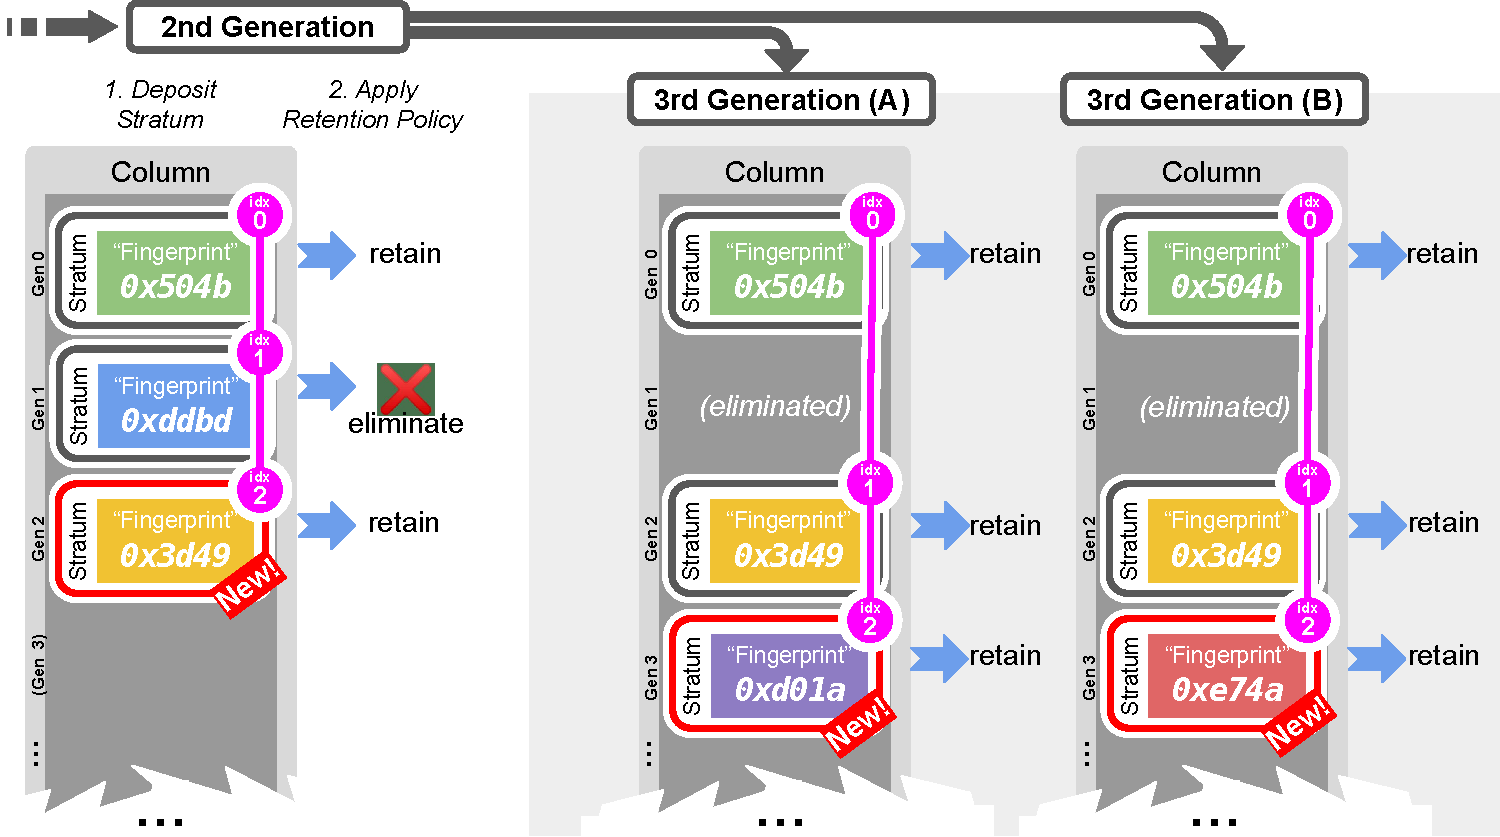
\includegraphics[width=\textwidth]{img/deposit-process}
  \end{minipage}%
  \begin{minipage}{0.4\textwidth}
    \caption{
    Cartoon illustration of stratum deposit process.
    This process marks the elapse of a generation when a hereditary stratigraphic column is inherited by an offspring.
    First, a new stratum is appended to the end of the column with a randomly-generated ``fingerprint.''
    This ``fingerprint'' distinguishes strata that were generated along disparate lines of descent (e.g., \texttt{0xd01a} for 3rd Generation A and \texttt{0xe74a} for 3rd generation B).
    Then, the column's configured stratum retention policy is applied to ``prune'' the column by eliminating strata from specific generations.
    Although this cartoon depicts an empty space for eliminated strata, the underlying data structure behind a column (i.e., the pink overlay) can condense to reduce space complexity.
    }\label{fig:deposit-process}
  \end{minipage}
\end{figure*}


However, as currently stated, under this algorithm fingerprints will accumulate proportionally to the length of evolutionary history simulated.
In an evolutionary run with tens of thousands of generations or more, this approach would soon become intractable --- particularly when columns are serialized and transmitted between distributed computing elements.
To solve this problem, we can trade off precision for compactness by deleting strata from columns as time progresses.
Figure \ref{fig:deposit-process} overviews how stratum deposit and stratum elimination progress over two generations under the hereditary stratigraphic column scheme.

Different patterns of deletion will lead to different trade-offs, both in terms of the scaling relationship of column size to generations elapsed and in terms of the arrangement of precision over evolutionary history (i.e., focusing precision on more recent evolutionary history versus spreading it evenly over the entire history).

We refer to the rule set used to selectively eliminate strata over time as the ``stratum retention policy.''
We explore several different retention policy designs here, and implement our software to allows for free, modular interchange of retention policies.
It is possible to define a policy through either of two mechanisms.
First, policy can be defined as a ``predicate'' where the generation of a stratum and the current number of strata deposited is passed into a function that returns whether that strata should be retained at that point in time.
Second, policy can be defined as a ``condemner'' generator where, given the current number of strata deposited, the set of ranks that should be deleted at this point in time are yielded.
Although the predicate form is useful for analyzing and proving properties of policies, the condemner form is generally more efficient in practice.
We provide predicate and condemner implementations for each stratum retention policy discussed here.

It should be noted that condemners and predicates are both defined in terms of stratum generation, not stratum index among retained strata in the column.
Therefore, it may seem necessary to store the generation of deposit within the stratum data structure.
However, it is not necessary to store this data with known total generations deposited you can map backwards from index to recover generation deposited.
We provide this formula for each stratum retention policy.
Finally, useful for anticipating memory usage within an experiment, for each policy we provide a formula to calculate the exact number of strata retained under any parameterization after $k$ generations.

\subsection{Fixed Resolution Stratum Retention Policy}
Important property: because they're deterministic, when you compare two columns that are unfolding with the same policy, every stratum that is held by the older column before the generation of the newer column is also guaranteed to be held by that newer column.


Likely wouldn't ,
We include it here for illustrative purposes.

First row in Figure \ref{fig:retention-policies}

\subsection{Depth-Proportional Resolution Stratum Retention Policy}

Second row in Figure \ref{fig:retention-policies}

This functor enacts the depth-proportional resolution policy by specifying
whether a stratum with deposition rank r should be retained within the
hereditary stratigraphic column after n strata have been deposited.

The depth-proportional resolution policy ensures estimates of MRCA rank will
have uncertainty bounds less than or equal to a user-specified
proportion of the largest number of strata deposited on either column.
Thus, MRCA rank estimate uncertainty scales as O(n) with respect to the
greater number of strata deposited on either column.

Under the depth-proportional resolution policy, the number of strata
retained (i.e., space complexity) scales as O(1) with respect to the number
of strata deposited.

Decide if a stratum within the stratagraphic column should be
retained or purged.

Every time a new stratum is deposited, this method is called on each
stratum present in a HereditaryStratigraphicColumn to determine whether
it should be retained. Strata that return False are immediately purged
from the column, meaning that for a stratum to persist it must earn a
True result from this method each and every time a new stratum is
deposited.

This functor's retention policy implementation guarantees that columns
will retain appropriate strata so that for any two columns with m and n
strata deposited, the rank of the most recent common ancestor can be
determined with uncertainty of at most

\begin{align*}
    bound = floor(max(m, n) / guaranteed_depth_proportional_resolution)
\end{align*}

ranks. Achieving this limit on uncertainty requires retaining sufficient
strata so that no more than bound ranks elapsed between any two strata.
This policy accumulates retained strata at a fixed interval until twice
as many as $guaranteed_depth_proportional_resolution$ are at hand. Then,
every other retained stratum is purged and the cycle repeats with a new
twice-as-wide interval between retained strata.

\subsection{Tapered Depth-Proportional Resolution Stratum Retention Policy}

Third row in Figure \ref{fig:retention-policies}

elaborated so that unnecessary are removed gradually from back to front as new instead.
This makes it easier for our experiments and likely would

Functor to implement the tapered depth-proportional resolution stratum
retention policy, for use with HereditaryStratigraphicColumn.

This functor enacts the tapered depth-proportional resolution policy by
specifying whether a stratum with deposition rank r should be retained
within the hereditary stratigraphic column after n strata have been
deposited.

The tapered depth-proportional resolution policy ensures estimates of MRCA
rank will have uncertainty bounds less than or equal to a user-specified
proportion of the largest number of strata deposited on either column.
Thus, MRCA rank estimate uncertainty scales as O(n) with respect to the
greater number of strata deposited on either column.

Under the tapered depth-proportional resolution policy, the number of strata
retained (i.e., space complexity) scales as O(1) with respect to the number
of strata deposited.

This policy accumulates retained strata at a fixed interval until twice
as many as $guaranteed_depth_proportional_resolution$ are at hand. Then,
every other retained stratum is purged gradually from back to front
until the cycle repeats with a new twice-as-wide interval between
retained strata.

\subsection{MRCA-Recency-Proportional Resolution Stratum Retention Policy}

Last row in Figure \ref{fig:retention-policies}

Functor to implement the MRCA-recency-proportional resolution stratum
retention policy, for use with HereditaryStratigraphicColumn.

This functor enacts the MRCA-recency-proportional resolution policy by
specifying whether a stratum with deposition rank r should be retained
within the hereditary stratigraphic column after n strata have been
deposited.

The MRCA-recency-proportional resolution policy ensures estimates of MRCA
rank will have uncertainty bounds less than or equal to a user-specified
proportion of the actual number of generations elapsed since the MRCA and
the deepest of the compared columns. MRCA rank estimate uncertainty scales
in the worst case scales as O(n) with respect to the greater number of
strata deposited on either column. However, with respect to estimating the rank of the MRCA when lineages diverged any fixed number of generations ago,
uncertainty scales as O(1).

Under the MRCA-recency-proportional resolution policy, the number of strata
retained (i.e., space complexity) scales as O(log(n)) with respect to the
number of strata deposited.

Decide if a stratum within the stratagraphic column should be
retained or purged.

Every time a new stratum is deposited, this method is called on each
stratum present in a HereditaryStratigraphicColumn to determine whether
it should be retained. Strata that return False are immediately purged
from the column, meaning that for a stratum to persist it must earn a
True result from this method each and every time a new stratum is
deposited.

This functor's retention policy implementation guarantees that columns
will retain appropriate strata so that for any two columns with m and n
strata deposited, the rank of the most recent common ancestor at rank k
can be determined with uncertainty of at most

\begin{align*}
    bound = floor(
        max(m - k, n - k)
        / guaranteed_mrca_recency_proportional_resolution
    )
\end{align*}

ranks.

How does the predicate work and how does it guarantee this resolution?

To begin, let's consider setting up just the *first* rank of the
stratum after the root ancestor we will retain.


% root ancestor                                     extant individual
% |                                                                 |
% |                    num_strata_deposited                         |
% | ___________________________/\_________________________________  |
% |/                                                               \|
% |-------------------|#############################################|
%  \_______  ________/|\____________________  ______________________/
%          \/         |                     \/
%    max_uncertainty  |            worst_case_mrca_depth
%                     |
%                     proposed retention rank

To provide guaranteed resolution, $max_uncertainty$ must be leq than

\begin{align*}
   worst_case_mrca_depth // guaranteed_resolution
\end{align*}

So, to find the largest permissible $max_uncertainty$ we must solve

\begin{align*}
   max_uncertainty = worst_case_mrca_depth // guaranteed_resolution
\end{align*}
By construction we have

\begin{align*}
   worst_case_mrca_depth = num_strata_deposited - max_uncertainty
\end{align*}
Substituting into the above expression gives

\begin{align*}
   max_uncertainty
   = (num_strata_deposited - max_uncertainty) // guaranteed_resolution
\end{align*}

Solving for $max_uncertainty$ yields

\begin{align*}
  max_uncertainty
  = num_strata_deposited // (guaranteed_resolution + 1)
\end{align*}

We now have an upper bound for the rank of the first stratum rank
we must retain. We can repeat this process recursively to select
ranks that give adequate resolution proportional to
$worst_case_mrca_depth$.

However, we must guarantee that these ranks are actually available for
us to retain (i.e., it hasn't been purged out of the column at a
previous time point as the column was grown by successive deposition).
We will do this by picking the rank that is the highest power of 2
less than or equal to our bound. If we repeat this procedure as we
recurse, we are guaranteed that this rank will have been preserved
across all previous timepoints.

This is because a partial sum sequence where all elements are powers
of 2 and elements in the sequence are will include all multiples of
powers of 2 greater than or equal to the first element that are less
than or equal to the sum of the entire
sequence.

An example is the best way to convince yourself. Thinking analogously
in base 10,

   100 + 10... + 1...

the partial sums of any sequence of this form will always include all
multiples of powers of 100, 1000, etc. that are less than or equal to
the sum of the entire sequence.

In our application, partial sums represent retained ranks. So, all
ranks that are perfect powers of 2 measuring from the root ancestor
will have been retained after being deposited. This property
generalizes recursively.

The calculation can be written mathematically as,

  weight of binary expansion of n (i.e., \#1's set in binary repr)
  + sum(
      floor( log2(n//r) )
      for r from 1 to r inclusive
  )
  + 1

where

\begin{align*}
  n = num_strata_deposited - 1
  r = resolution
\end{align*}

This expression for exact number deposited was extrapolated from
    * resolution = 0, <https://oeis.org/A063787> \citep{sloane2021a063787}
    * resolution = 1, <https://oeis.org/A056791> \citep{sloane2021a056791}
and is unit tested extensively.

\subsection{Computational Experiments}

In order to assess the hereditary stratigraph approach in an applied setting, we simulated the process of stratigraph propagation over known ``ground truth'' phylogenies extracted from pre-existing digital evolution simulations.
These simulations propagated populations of between X and Y bitstrings between 3,000 and 5,000 generations under the NK fitness landscape model (TODO cite).
In order to ensure coverage of a variety of phylogenetic conditions, we sampled a variety of selection schemes that impose profoundly different ecological regimens (cite Emily's paper).
We used five data sets:
\begin{itemize}
  \item EcoEA Selection,
  \item Lexicase Selection,
  \item Random Selection,
  \item Tournament Selection, and
  \item TODO missing one.
\end{itemize}

Supplementary Table TODO provides full details on the configured conditions of each run.
The phylogenies themselves are available in our data repository for this project.


\subsection{Software and Data}

A prototype of this approach has been implemented \url{https://github.com/mmore500/dishtiny/blob/incoming/include/dish2/genome/PhyloFingerprints.hpp} and preliminarily tested \url{https://github.com/mmore500/dishtiny/blob/incoming/tests/dish2/genome/PhyloFingerprints.cpp}.

A Python library has been published with extensive documentation and unit testing on GitHub at \url{https://github.com/mmore500/hstrat} and on PyPI at \url{https://pypi.org/project/hstrat/}.
In the near future, we intend to complete and publish a corresponding C++ library.

We used many open source libraries in this work:
* \citep{sukumaran2010dendropy}
* \citep{cock2009biopython}
* \citep{virtanen2020scipy}
* \citep{hunter2007matplotlib}
* \citep{virtanen2020scipy}
* \citep{waskom2021seaborn}
* D3?

All supporting materials on GitHub at \url{https://github.com/mmore500/hereditary-stratigraph-concept} and notebooks are available for in-browser use via BinderHub at \url{https://mybinder.org/v2/gh/mmore500/hereditary-stratigraph-concept/HEAD?labpath=binder%2F} \citep{ragan2018binder}.
Data used in this work is available via the Open Science Framework at
\url{https://osf.io/4sm72/} \citep{hstratconceptsupplement} \citep{foster2017open}.

Our data is made available in the Alife Community Data Standards format TODO cite.

% \pragmaonce

% adapted from https://www.overleaf.com/learn/latex/Commands
\providecommand{\dissertationelse}[2]{%
% adapted from https://tex.stackexchange.com/a/33577
\ifdefined\DISSERTATION
#1
\else
#2
\fi
}

../../tex/lib/dissertationonly.tex

\begin{figure*}
  \centering
  \dissertationonly{\footnotesize}
  \begin{tabular}{m{0.05\textwidth}@{}|c@{}|c@{\hskip 0.01\textwidth}|m{0.14\textwidth}}
%-------------------------------------------------------------------------------
\hspace{-1ex}Policy&Lower-Resolution Parameterization&Higher-Resolution Parameterization&\makecell[c]{Properties}\\\hline
%-------------------------------------------------------------------------------
    \rotatebox{90}{\textbf{Fixed Resolution}}
  &
    \makecell{
      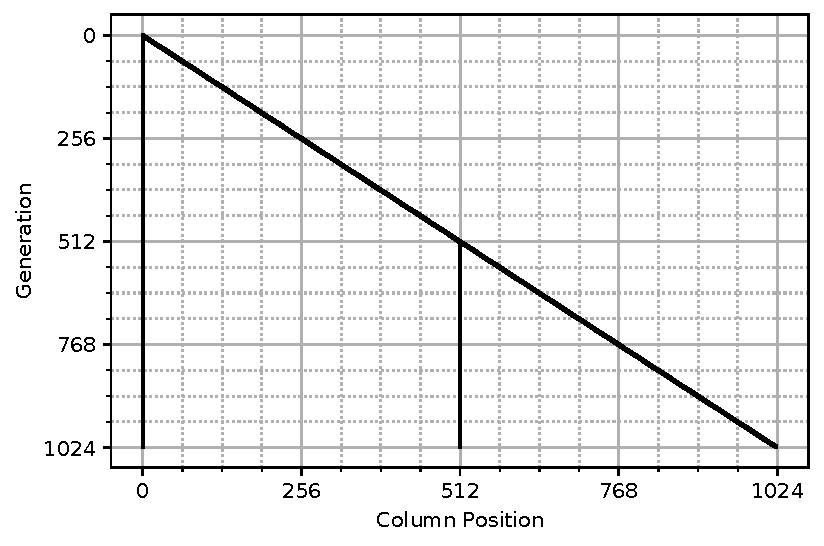
\includegraphics[valign=t,width=\dissertationelse{0.3}{0.4}\textwidth]{submodules/hereditary-stratigraph-concept/binder/retention-policies/teeplots/fixed_resolution=512+num_layers=1024+stratum_retention_predicate=fixed-resolution+viz=tweaked-stratum-retention-drip-plot+ext=}
    }
  &
    \makecell{
      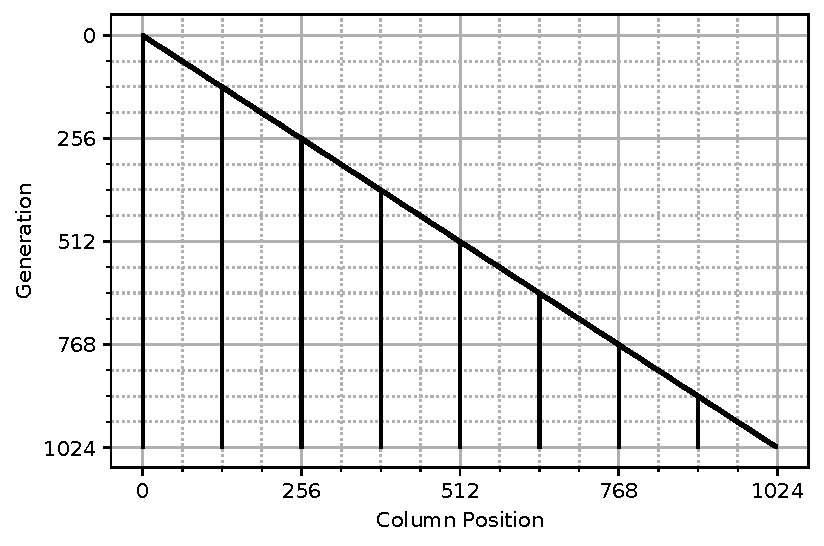
\includegraphics[valign=t,width=\dissertationelse{0.3}{0.4}\textwidth]{submodules/hereditary-stratigraph-concept/binder/retention-policies/teeplots/fixed_resolution=128+num_layers=1024+stratum_retention_predicate=fixed-resolution+viz=tweaked-stratum-retention-drip-plot+ext=}
    }
  &
  \makecell[{{p{0.14\textwidth}}}]{
  \centering
    \bf{Space Complexity}\\
    $O(n)$\\
    \bf{MRCA Uncertainty}\\
    $O(1)$
  }
  \makecell[{{p{0.14\textwidth}}}]{
  \raggedright
    where $n$ is gens elapsed.
  }\\\hline
%-------------------------------------------------------------------------------
    \adjustbox{
      minipage=10em,
      rotate=90,
    }{
      \centering
      \textbf{Depth-Proportional Resolution}
      \par
    }
  &
    \makecell{
      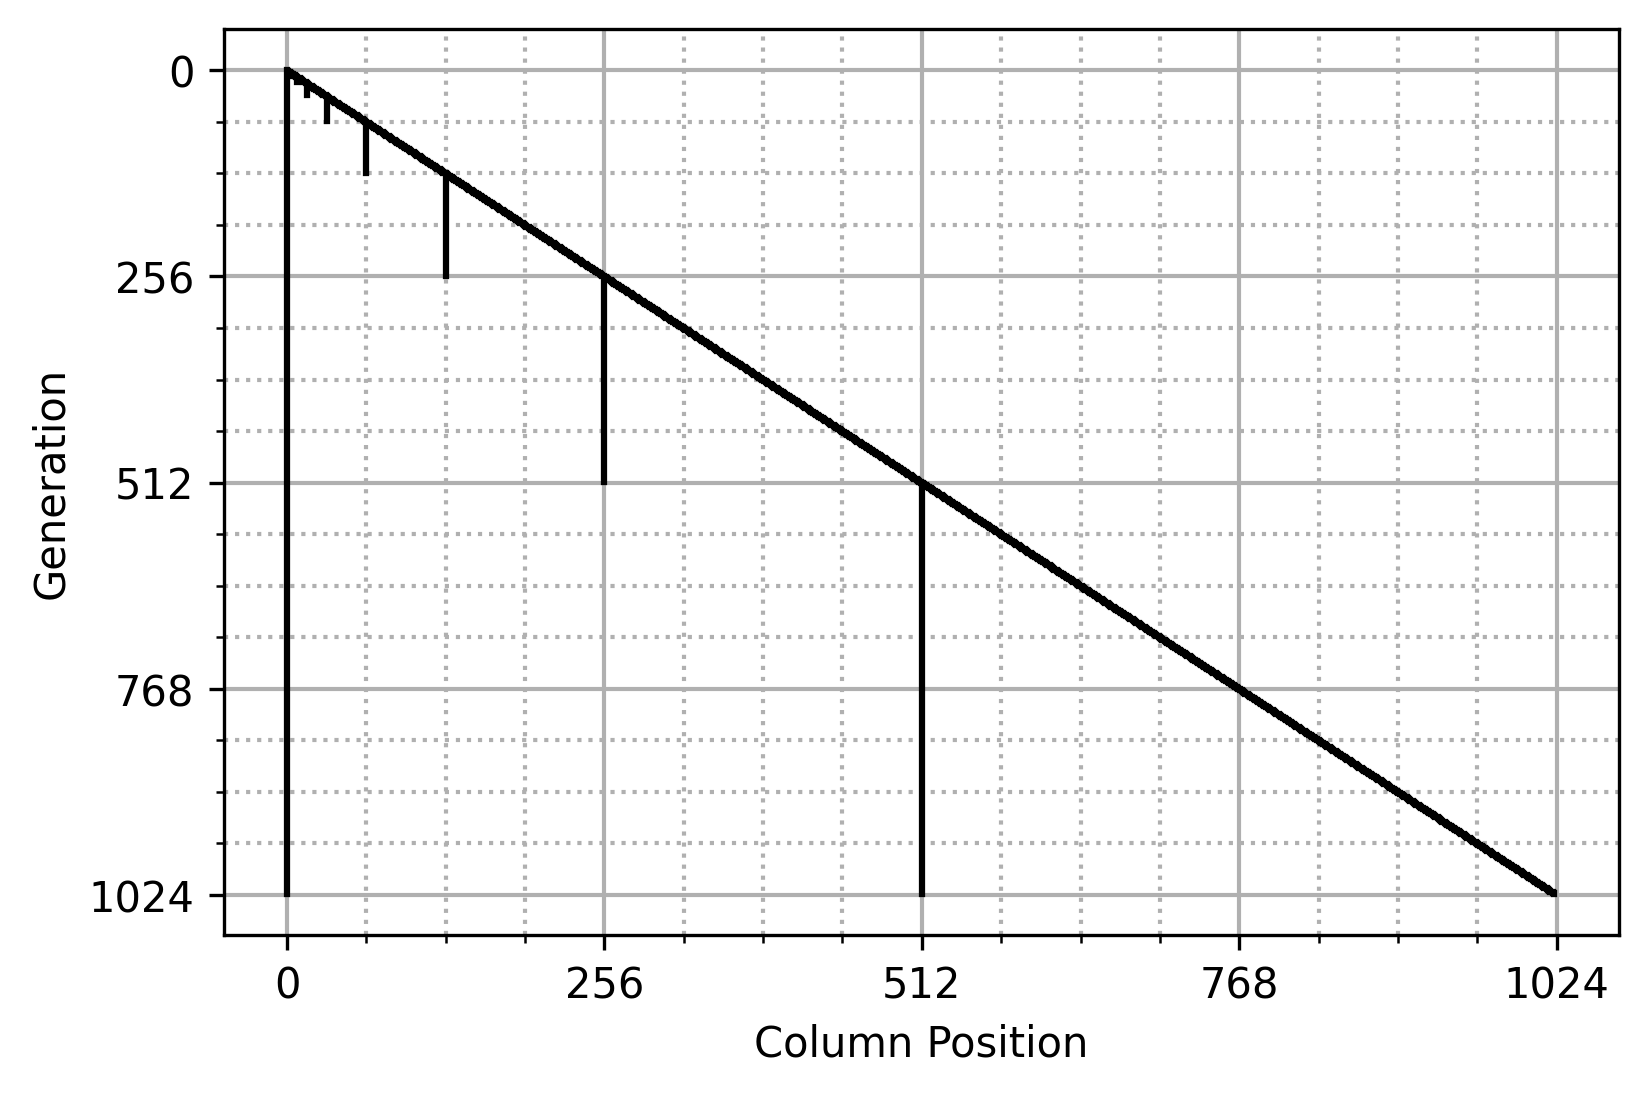
\includegraphics[valign=t,width=\dissertationelse{0.3}{0.4}\textwidth]{submodules/hereditary-stratigraph-concept/binder/retention-policies/teeplots/guaranteed_depth_proportional_resolution=1+num_layers=1024+stratum_retention_predicate=depth-proportional-resolution+viz=tweaked-stratum-retention-drip-plot+ext=}
    }
  &
    \makecell{
      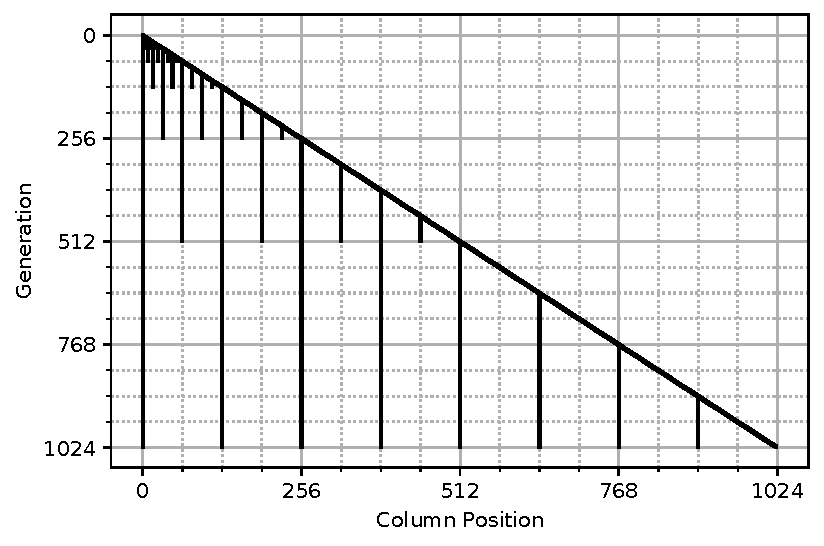
\includegraphics[valign=t,width=\dissertationelse{0.3}{0.4}\textwidth]{submodules/hereditary-stratigraph-concept/binder/retention-policies/teeplots/guaranteed_depth_proportional_resolution=4+num_layers=1024+stratum_retention_predicate=depth-proportional-resolution+viz=tweaked-stratum-retention-drip-plot+ext=}
    }
  &
  \makecell[{{p{0.14\textwidth}}}]{
  \centering
    \bf{Space Complexity}\\
    $O(1)$\\
    \bf{MRCA Uncertainty}\\
    $O(n)$
  }
  \makecell[{{p{0.14\textwidth}}}]{
  \raggedright
    where $n$ is gens elapsed.
  }\\\hline
%-------------------------------------------------------------------------------
    \adjustbox{
      minipage=15em,
      rotate=90,
    }{
      \centering
      \textbf{Tapered Depth-Proportional Resolution}
      \par
    }
  &
    \makecell{
      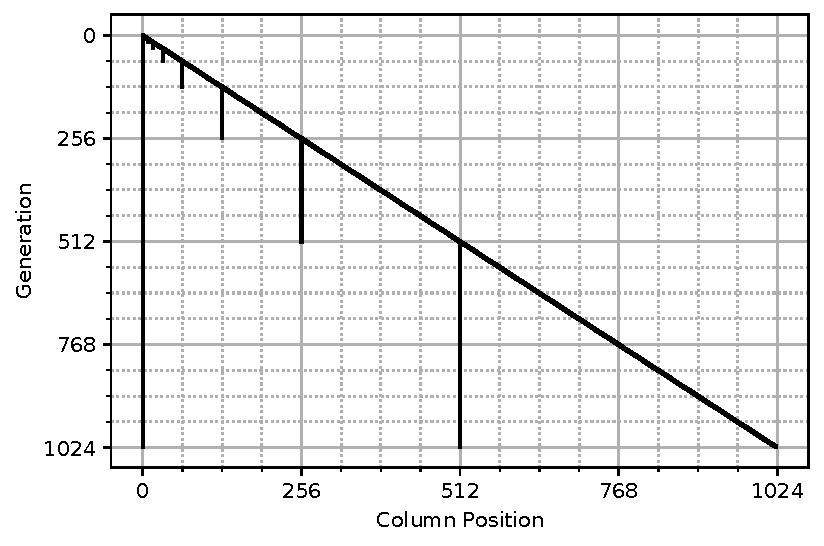
\includegraphics[valign=t,width=\dissertationelse{0.3}{0.4}\textwidth]{submodules/hereditary-stratigraph-concept/binder/retention-policies/teeplots/guaranteed_depth_proportional_resolution=1+num_layers=1024+stratum_retention_predicate=tapered-depth-proportional-resolution+viz=tweaked-stratum-retention-drip-plot+ext=}
    }
  &
    \makecell{
      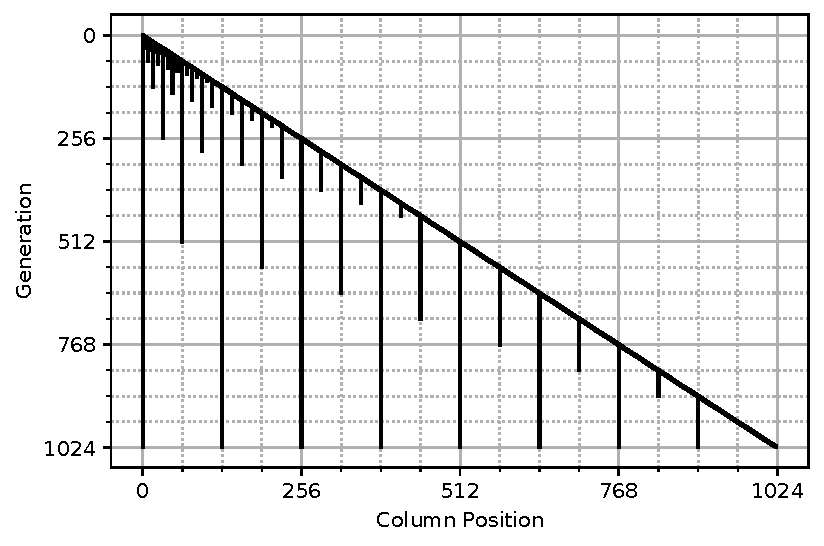
\includegraphics[valign=t,width=\dissertationelse{0.3}{0.4}\textwidth]{submodules/hereditary-stratigraph-concept/binder/retention-policies/teeplots/guaranteed_depth_proportional_resolution=4+num_layers=1024+stratum_retention_predicate=tapered-depth-proportional-resolution+viz=tweaked-stratum-retention-drip-plot+ext=}
    }
  &
  \makecell[{{p{0.14\textwidth}}}]{
  \centering
    \bf{Space Complexity}\\
    $O(1)$\\
    \bf{MRCA Uncertainty}\\
    $O(n)$
  }
  \makecell[{{p{0.14\textwidth}}}]{
  \raggedright
    where $n$ is gens elapsed.
  }\\\hline
%-------------------------------------------------------------------------------
  \adjustbox{
    minipage=15em,
    rotate=90,
  }{
    \centering
    \textbf{Recency-Proportional\\Resolution}
    \par
  }
  &
  \makecell{
    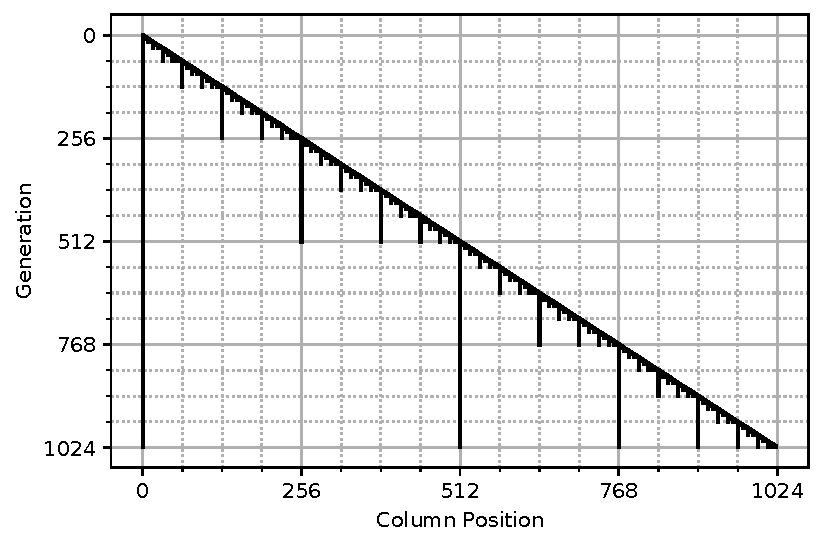
\includegraphics[valign=t,width=\dissertationelse{0.3}{0.4}\textwidth]{submodules/hereditary-stratigraph-concept/binder/retention-policies/teeplots/guaranteed_mrca_recency_proportional_resolution=0+num_layers=1024+stratum_retention_predicate=recency-proportional-resolution+viz=tweaked-stratum-retention-drip-plot+ext=}
  }
  &
  \makecell{
    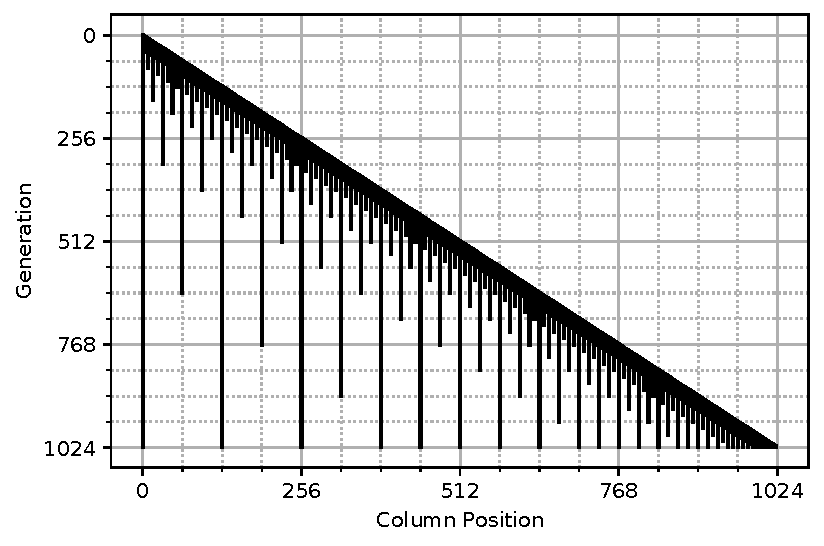
\includegraphics[valign=t,width=\dissertationelse{0.3}{0.4}\textwidth]{submodules/hereditary-stratigraph-concept/binder/retention-policies/teeplots/guaranteed_mrca_recency_proportional_resolution=4+num_layers=1024+stratum_retention_predicate=recency-proportional-resolution+viz=tweaked-stratum-retention-drip-plot+ext=}
  }
  &
  \makecell[{{p{0.14\textwidth}}}]{
  \centering
  \bf{Space Complexity}\\
  $O(\log(n))$\\
  \bf{MRCA Uncertainty}\\
  $O(m)$
  }
  \makecell[{{p{0.14\textwidth}}}]{
  \raggedright
  where $m$ is gens since MRCA and $n$ is total gens elapsed.
  }\\


  \end{tabular}
  \caption{
  Comparison of stratum retention policies.
  Policy visualizations show retained strata in black.
  Time progresses along the $y$-axis from top to bottom.
  New strata are introduced along the diagonal and then ``drip'' downward as a vertical line until eliminated.
  The set of retained strata present within a column at a particular generation $g$ can be read as intersections of retained vertical lines with a horizontal line with intercept $g$.
  Policy visualizations are provided for two parameterizations for each policy: the first where the maximum uncertainty of MRCA generation estimates would be 512 generations and the second where the maximum uncertainty of MRCA generation estimates would be 128 generations.
  }
  \label{fig:retention-policies}
\end{figure*}




\begin{figure*}
  \centering
    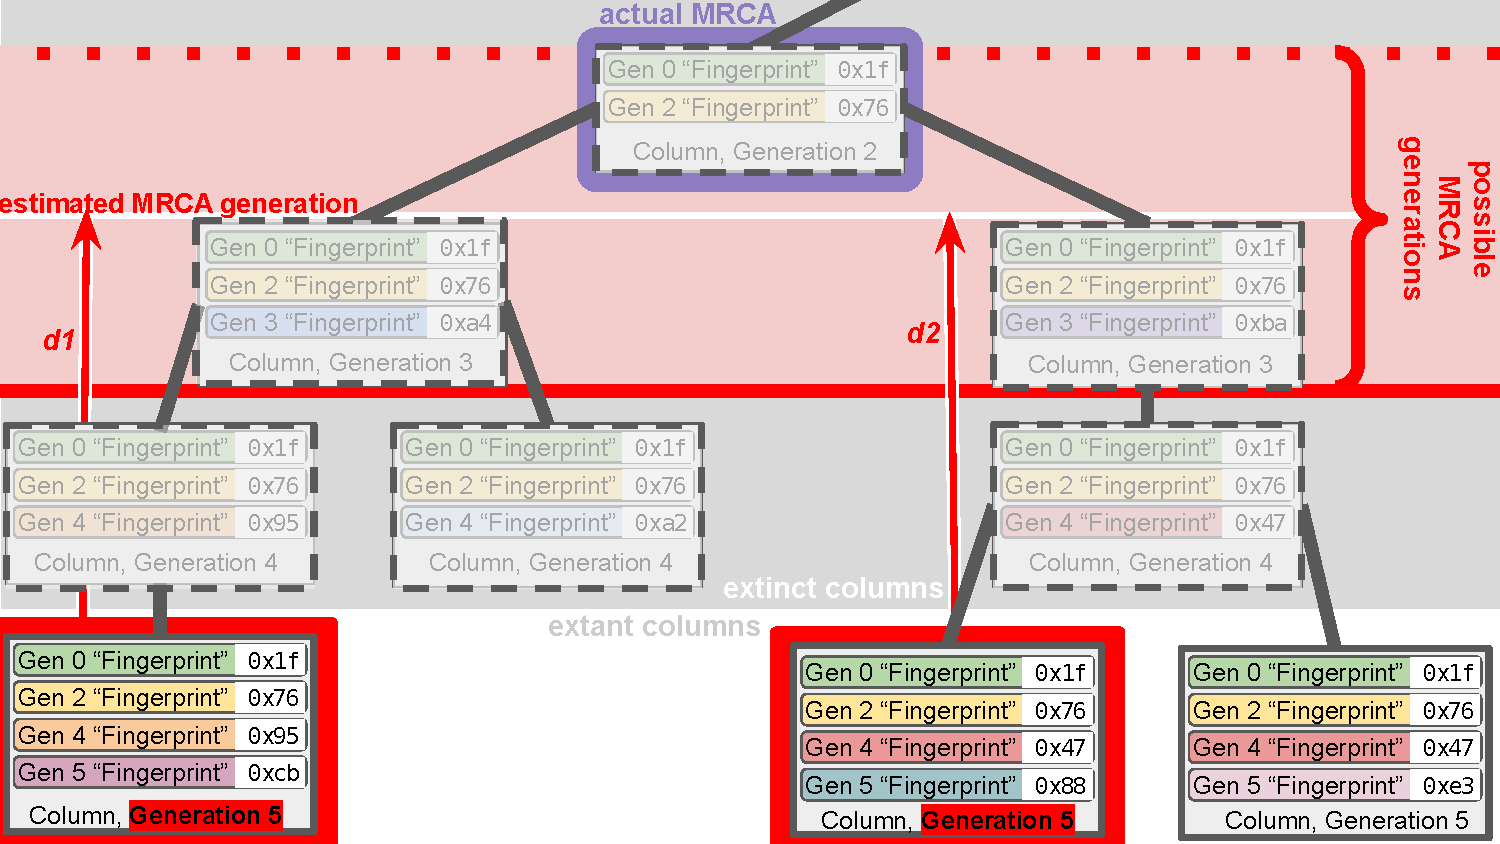
\includegraphics[width=\textwidth]{img/phylogenetic-inference}
    \caption{
    Cartoon illustration of column inheritance along a phylogenetic tree and the process to infer phylogenetic history along extant columns.
    This scenario supposes a stratum retention policy where only strata from even generations are retained.
    The common ancestor of the focal clade, which is at generation 2, is shown at top.
    Generation 3 columns inherit that ancestor's strata and each append a new stratum.
    Generation 4 columns append another new stratum then eliminate their generation 3 strata.
    Finally, another generation elapses to yield generation 5 strata.
    Suppose that only generation 5 strata are extant.
    So, greyed-out columns above are not directly observable.
    Phylogenetic history is deduced by pairwise comparison between extant columns.
    For each pair (like the example highlighted in red) a phylogenetic distance can be computed as the sum generations elapsed to each extant column after the estimated generation of their MRCA.
    These pairwise distances can then be fed into a phylogeny reconstruction algorithm.
    }
  \label{fig:phylogenetic-inference}
\end{figure*}

